Este capítulo apresenta o problema identificado, a proposta de resolução para este problema, o planejamento de ações para alcançar a solução e os resultados que são esperados ao fim da pesquisa.



\section{Metodologia}
\label{sec:methodology}

 Para a resolução do problema apresentado, é proposto a criação de uma ontologia que contemple as propriedades necessárias de pacientes a serem atendidos em uma especialidade médica e um protótipo que utilize esses itens e gerencie uma fila de espera de acordo com critérios preestabelecidos por médicos.
 
 Como forma de obter um primeiro protótipo para resolução de problemas da área da saúde utilizando tecnologias da web semântica, foi desenvolvido uma aplicação com o objetivo de extrair os termos presentes em hemogramas em formato PDF baseados em texto e relacionar cada termo extraído com a terminologia LOINC, permitindo que dados a princípio tabulares, pudessem após essa tratativa, serem compreendidos  pelos computadores.

    Com o intuito de validar a proposta, será desenvolvido um estudo de caso com o Hospital das Clínicas da Faculdade de Medicina de Marília (HCFAMEMA), onde se espera implantar a ontologia e o protótipo. Médicos desse hospital avaliarão o gerenciamento realizado pelo protótipo. Eles informarão qual sua concordância com a fila de atendimento gerada pelo protótipo (de acordo com a quantidade de pacientes que julgarem estar corretamente posicionados) e, para efeito de comparação, também informarão sua concordância com a fila de atendimento atualmente usada pelo hospital (para o mesmo conjunto de pacientes). Nosso objetivo é determinar se o protótipo pode, de fato, gerenciar uma fila de espera de forma tão (ou mais) eficaz que o que é feito atualmente no hospital segundo a visão de especialistas (médicos).
	
	O intuito não é discutir quais devem ser os critérios a serem utilizados pelos médicos para avaliar se um paciente X tem prioridade em relação ao paciente Y, mas sim possibilitar que, a partir de critérios previamente estabelecidos, o computador possa fazer essa triagem de forma tão (ou mais) eficaz que os funcionários que hoje desempenham essa tarefa. O objetivo é permitir um ordenamento mais próximo ao que os médicos aconselham, levando a uma fila de atendimento mais justa e transparente. 
	
	O método para se chegar ao objetivo desta pesquisa é utilizar recursos da web semântica, como ontologias, para que se possa representar características de pacientes que poderão ser utilizados para gerenciar uma fila de espera. Devido as restrições de tempo de um trabalho de mestrado, o protótipo desenvolvido vai se restringir a uma especialidade médica específica. Isso visa reduzir o escopo da ontologia a ser desenvolvida e o tempo de desenvolvimento do protótipo.

    \section{Cronograma}

	Considerando um tempo de 25 meses para o desenvolvimento da pesquisa proposta e a numeração das tarefas apresentadas na \autoref{sec:methodology}, o cronograma das atividades se apresenta na Tabela 1 %\autoref{tab:cronogram}.
	
	  \begin{enumerate}
    	\item Conclusão da validação do exame de proficiência em língua estrangeira;
        \item Integralização dos créditos obrigatórios;
        \item Mapeamento da literatura;
        \item Elaboração e apresentação dos artefatos relacionados ao exame de qualificação;
         \item Desenvolvimento da ontologia OWL que represente indicadores para classificação de prioridades para o atendimento de uma especialidade médica;
        \item Desenvolvimento e testes de um protótipo que utilize a ontologia desenvolvida e gerencie uma fila de espera utilizando critérios definidos;
        \item Elaboração e submissão de artigos;
        \item Elaboração e apresentação dos artefatos relacionados a defesa;
    \end{enumerate}
    
    \begin{table}[htbp]
    	\centering
        \caption{Cronograma das atividades da pesquisa.}
        \label{tab:cronogram}
        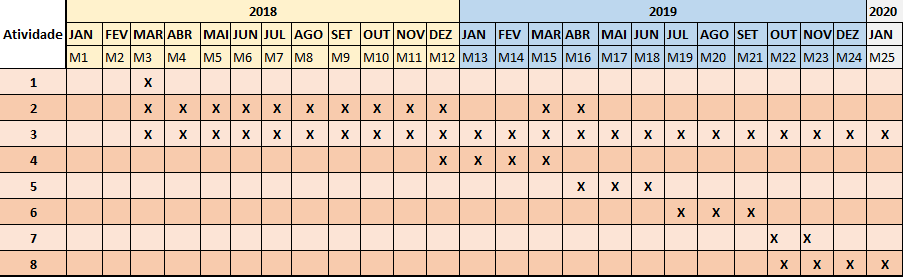
\includegraphics[width=1\linewidth]{images/cronogram}
        \fautor
    \end{table}
    
    \pagebreak
    
   \section{ Resultados Esperados}

	Ao final desta pesquisa espera-se as seguintes contribuições:
	
	\begin{itemize}
		\item Uma ontologia OWL que represente indicadores para classificação de prioridades para o atendimento de uma especialidade médica;
        \item  Um protótipo que gerencie filas de espera computacionalmente e se mostre  mais eficaz que o gerenciamento atual do HC FAMEMA;
        \item Estudo de caso que mostre que o modelo proposto pode auxiliar na gestão de filas do Sistema Único de Saúde (no HC FAMEMA) e ter benefícios se comparado a outras formas de gerenciamento;
	\end{itemize}
